
\begin{figure}

\caption{Three-Dimensional Tissue Reconstruction via 3DimViewer}
\label{fig:rad2}

\begin{tikzpicture}
%\nodeincludegraphicsTR{2.7cm}{2cm}{pics/RAD-2.png}

\node[inner sep=0pt] (r2) at (0,0)
    {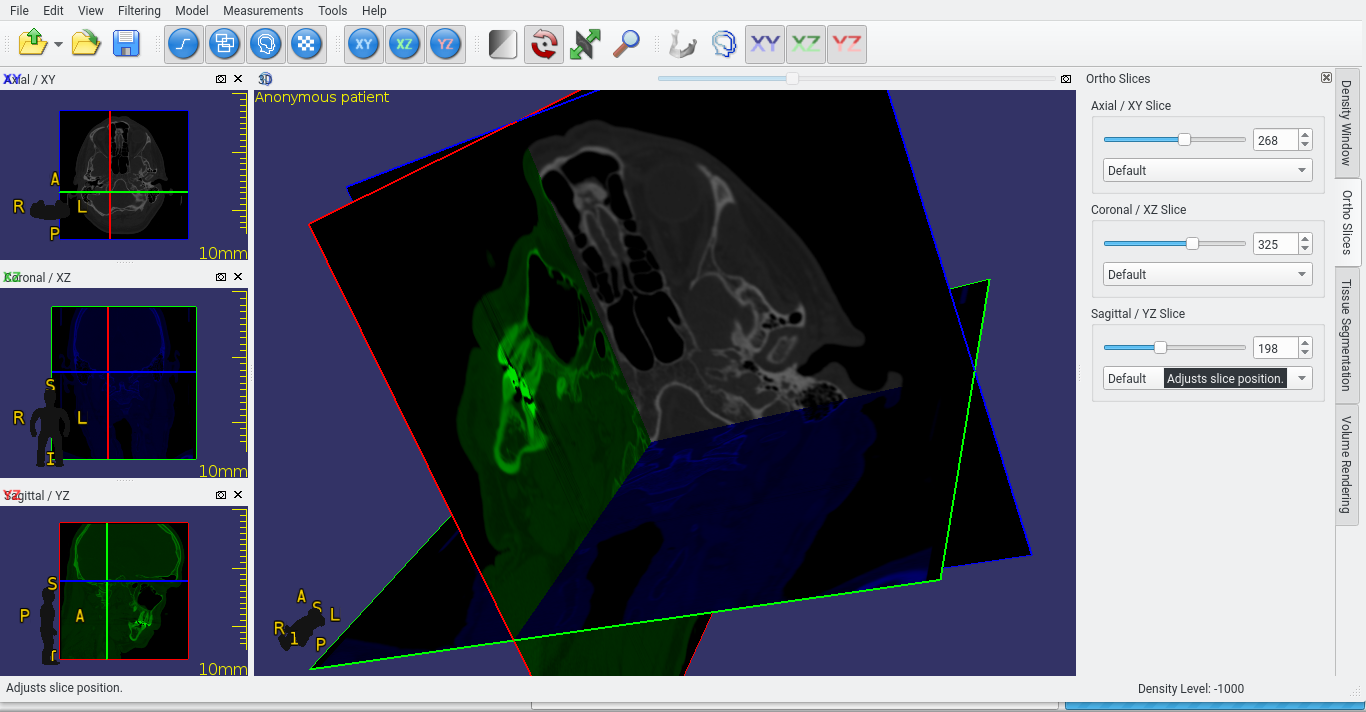
\includegraphics[width=7in, 
    	trim={0mm 0mm 0mm 0mm},clip]
    	{pics/Rad-2.png}};


 \node [anchor=west,fill=brown!20!white,inner sep=7, text width=14cm]
  (longnote) at (-6.5,-4.5) {%\vspace{-8pt}%  %{\color{rb!85!red}{
  {\textbf{3DimViewer builds 3D models from 
2D radiology image series ...}}};

\end{tikzpicture}


\end{figure}

